
\documentclass[conference]{IEEEtran}

\usepackage[utf8]{inputenc}
\usepackage[T1]{fontenc}
\usepackage{lmodern} % load a font with all the characters
\usepackage{xcolor}
\usepackage{multicol}
\usepackage{graphicx}
\usepackage{subfig}
\usepackage{afterpage}
\graphicspath{ {images/} }
\newcommand\myworries[1]{\textcolor{red}{#1}}

\usepackage{abstract}
\renewcommand{\abstractname}{}    % clear the title

% correct bad hyphenation here
\hyphenation{op-tical net-works semi-conduc-tor}


\begin{document}

\title{Trabalho de Algoritmos Genéticos\\ Parte 2}


\author{\IEEEauthorblockN{Fábio Beranizo Fontes Lopes}
\IEEEauthorblockA{Escola de Artes, Ciências e Humanidades (EACH)\\
Universidade de São Paulo (USP)\\
Email: f.lopes@usp.br}
}

% make the title area
\maketitle

% As a general rule, do not put math, special symbols or citations
% in the abstract
\begin{abstract}
Este relatório apresenta a discussão da parte 2  do trabalho de algoritmos
genéticos (GA) para a disciplina de Inteligência Computacional. Foi avaliada a
utilização de GA para roteamento de veículos. O foco se manteve em
analisar o comportamento do algoritmo mediante a utilização de
diferentes técnicas, operadores e parametrizações.\\
O trabalho foi desenvolvido utilizando a linguagem de programação Python,
especificamente sua distribuição Anaconda.\\
\end{abstract}

% no keywords

\section{Problema de Roteamento de Veículos}
O problema de roteamento de veículos (VRP) é o nome dado a uma classe de problemas em que rotas de veículos são otimizadas para servir um grupo de clientes. Determinar a solução ótima é um problema NP-difícil, assim é limitado o tamanho das instâncias que tem solução ótima rapidamente calculada. Isto tudo faz deste um problema interessante para ser solucionado por heurísticas, como o algoritmo genético utilizado neste trabalho.\\

Existem muitas variações para o VRP:
\begin{itemize}
\item CVRP (Capacitated VRP): os veículos possuem capacidade limitada
\item VRPTW (VRP with time windows): cada cliente tem que ser atendido dentro de uma janela de tempo
\item MDVRP (Mutliple Depot VRP): múltiplos depósitos são usados para atender os clientes
\item VRPPD (VRP with Pick-up and Delivering): clientes podem devolver produtos para o depósito
\item SDVRP (Split Delivery VRP): mais de um veículo pode atender um cliente
\item PVRP (Periodic VRP): as entregas podem ser feitas em alguns dias
\item OVRP (Open VRP): os veículos não precisam voltar ao depósito
\end{itemize}

Neste trabalho a variação de VRP avaliada foi o CVRP. Neste problema, uma quantidade de veículos com capacidade uniforme deve servir demandas de clientes com custo mínimo de deslocamento. Uma descrição mais formal deste problema se encontra a seguir:\\

Objetivo: Minimizar a frota de veículos e a soma das distâncias de viagem. A demanda total para cada rota 
não pode exceder a capacidade do veículo que serve essa rota.

Factibilidade: A solução é factível se a demanda total atribuída a cada rota não excede a capacidade do veículo que serve à rota.

Formulação:
\begin{itemize}
    \item Seja $V = \{v_{0}, v_{1},\ldots , v_{n}\}$ um conjunto de vértices tal que:
    \begin{itemize}
    \item Um depósito está localizado em $v_{0}$
    \item $V' = V \backslash \{v_{0}\}$ é um conjunto de $n$ clientes
    \end{itemize}

\item $A_ij = {(v_i,v_j)/v_i,v_j \in V}$ é um conjunto de arestas.
\item $C$ é uma matriz de distâncias não negativas $c_{ij}$ entre clientes $v_i$ e $v_j$
\item $d$ é um vetor de demandas de clientes
\item $R_{i}$ é a rota para o veículo $i$
\item $m$ é o número de veículos. Cada rota é atribuída a cada veículo
\item $Q$ é a capacidade de um veículo
\end{itemize}

Uma solução factível é composta de:
\begin{itemize}
\item uma partição ${R_{1},\ldots ,R_{m}}$ de $V$
\item uma permutação $\sigma_{i}$ de $R_{i}\bigcup {0}$ especificando a ordem dos clientes na rota $i$
\end{itemize}

O custo de uma dada rota ($R_i = \{v_0,v_1,...,v_{m+1}\}$), onde $v_i \in V$ e $v_0 = v_{m+1} = 0$, é dado por: $F(R_{i})=\sum_{i=0}^{m} c_{i,i+1} + \sum_{i=1}^{m} \delta _{i}$. 

A demanda total de todos os clientes servidos em uma rota $R_{i}$ não excede a capacidade do veículo $Q$: $\sum_{i=1}^{m} d_{i} \leq Q$.

\section{Algoritmo Genético}
Algoritmos Genéticos (GA) são heurísticas inspiradas na seleção natural biológica. GA gera soluções aproximadas para um dado problema, buscando melhorar os resultados a cada geração. Utilizando soluções antigas (pais) e certos operadores, são criadas novas soluções (filhos).

\subsection{Operadores Genéticos}
Indivíduos selecionados de uma população passam por um dos 3 tipos de operadores genéticos: reprodução, crossover e mutação. Neste trabalho foram analisados tipos de crossover e de mutação clássicos, além de outros orientados ao VRP.\\

\subsubsection{Seleção de Indivíduos}
Somente um operador de seleção de indivíduos foi analisado neste trabalho, o método da roleta. Ele operador foi escolhido por ser de fácil implementação e por apresentar bons resultados segundo a literatura. No entanto, durante o desenvolvimento foi possível perceber um problema: este operador aumenta consideravelmente o tempo de execução do algoritmo para grandes populações, uma vez que todos os indivíduos participam do sorteio.\\
O método da roleta leva em consideração o fitness de um indivíduo em relação ao fitness total da população. Nesse processo cada indivíduo possui uma probabilidade de ser selecionado (uma fatia da roleta) proporcional ao seu fitness. Embora não garanta que as melhores soluções sobrevivam, este método dá maiores probabilidades de sobrevida às soluções com bom fitness.

\subsubsection{Reprodução}
O operador de reprodução consiste em manter vivos alguns indivíduos baseados em seu fitness. Quanto melhor o fitness, maior a chance de sobrevivência.

\subsubsection{Crossover}
O operador crossover permite a criação de novos indivíduos a partir de organismos pais. Os descendentes possuem genótipo de ambos pais, embora geralmente sejam diferentes. O crossover é uma forma de ampliar o espaço de busca por soluções, porém mantendo-se material genético de boa qualidade de gerações anteriores.

\subsubsection{Mutação}
O operador de mutação permite inserir diversidade genética entre gerações de indivíduos trocando o valor de genes no cromossomo. Com maior variedade genética o espaço de busca é ampliado, possibilitando sair de situações de mínimo local.


% Aplicando operadores clássicos: esses são os operadores da parte I do trabalho. Esses operadores vão gerar muitas soluções infactíveis. Vocês devem analisar essa infactibilidade, mostrando como ela ocorre e por que. Discutam suas observações.
% b) aplicando operadores de correção: esses operadores são novos operadores, que vocês devem criar (há pelo menos um na bibliografia disponibilizada), para corrigir a infactibilidade criada na letra 

% TODO explicar operadores da primeira parte (crossover de um ponto, uniforme)

\subsection{Cromossomo}
O modelo de genótipo escolhido foi uma vetor que guarda a sequencia de clientes servidas por um veículo, e separada por um caracter ``X'' que representa o início de um outro veículo.

A escolha deste modelo de cromossomo foi devida a facilidade de manipulação do mesmo. Dessa forma, foi simples de executar os operadores de crossover e mutação bem como no cálculo de fitness.

No entanto, esse modelo de cromossomo facilitou a geração de solução infactíveis, como será explicado na próxima seção.

\begin{figure}[!t]
\centering
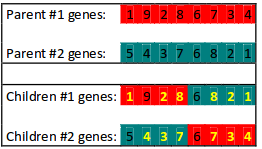
\includegraphics[width=2.5in]{error_in_crossover}
% where an .eps filename suffix will be assumed under latex, 
% and a .pdf suffix will be assumed for pdflatex; or what has been declared
% via \DeclareGraphicsExtensions.
\caption{Crossover que gera solução infactível.}
\label{fig_sim}
\end{figure}

\subsection{Problemas com operadores}
Durante o desenvolvimento da solução, foi detectado que a aplicação dos operadores de mutação e de crossover poderia criar soluções infactíveis para o problema. Para um cromossomo cujos genes representam um caminho, a aplicação de crossover leva fatalmente à geração de caminhos incompletos. A figura 1 mostra um exemplo de crossover que gera solução infactível. \\

Para contornar este problema uma primeira abordagem tomada foi repetir a realização do crossover por quantas vezes quanto necessário até que seja gerado um crossover válido. No entanto, após a realização de testes esta possibilidade foi descartada, uma vez que demorava muito até que surgisse uma solução válida. Além disso, muito recurso computacional era disperdiçado, fazendo com que essa solução fosse inviável. Assim, foi necessário buscar alternativas na literatura para resolver o problema.

% We also have to permutate the parents to find the fittings ones, and it is not sure, that we will find them. This is also rather time consuming and resource consuming


%A primeira solução adotada foi não realizar crossover. Foram analizadas diferentes combinações de população e porcentagens de reprodução e de mutação. Esta abordagem foi capaz de gerar soluções factíveis, porém a qualidade foi muito aleatória em cada execução.

\subsection{Simple Random Mutation}
A primeira solução escolhida observando-se a literatura foi o Simple Random Mutation (SRM).\\
O operador inicia selecionando aleatoriamente um cliente. O cliente é então removido de sua rota para evitar ficar duplicado na solução. A seguir é executada a função \textit{BestInsertion} que retorna o índice que indica o melhor lugar para inserir o cliente removido. O cliente é então inserido na posição retornada por best-insertion. \\

BestInsertion estima o custo para inserir uma subrota k1..kn entre dois clientes m e m+1 como: \[c = dist(m; m+1) - dist(m,k1) - dist(kn, m+1)\]
Os cliente m e m+1 que maximizam c são então escolhido para inserção da subrota.\\

\textbf{Essa técnica não verifica se a solução continua factível}, pois não verifica se a nova rota excede as capacidades do veículo.

\begin{verbatim}
Mutation(offspring, pSame)
NR <- number of routes in offspring
jMut <- random(0,NR)
RL <- number of customers in route jMut
kMut <- random(0,RL)
custo <- offspring[jMut][kMut]

delete cust from jMut
prob <- random(1,100)
if prob < pSame
  bestInd <- [jMut,BestInsertion(cust,jMut)]
else do j <- random(0,NR)
      while j = jMut
        bestInd <- [j, BestInsertion(cust,j)]
insertCust(cust, bestInd)
return offspring
\end{verbatim}

\subsection{Simple Random Crossover}
A técnica de Simple Random Crossover (SRC) é análoga a SRM. Dados 2 cromossomos P1 e P2, é feita a seleção de uma subrota de P2. Em seguida, os elementos da subrota são removidos de P1. A função BestInsertion é executada então em P1 e, na posição retornada é feita a inserção da subrota.

\begin{verbatim}
SRCrossover(P1,P2)
copy individual P1 into offspring
randomly select a subroute from P2
delete the members of the subroute from the offspring
bestInd <- BestInsertion(offspring, subroute)
insertSubRoute(offspring, bestInd, subroute)
return offspring
\end{verbatim}

\section{Função Fitness}
Para avaliar a seleção natural, cada indivíduo é avaliado em termos de seu valor de fitness. Essa medida, mede a qualidade das soluções e permite sua comparação.

Na parte 1 do trabalho o tipo do problema não exigiu muito trabalho de acerto da função de fitness. No entanto, nessa parte foi necessário contornar várias dificuldades, por exemplo: avaliar soluções infactíveis.\\
A forma adotada neste trabalho para lidar com soluções infactíveis foi somar um valor de penalidade ao fitness da solução.\\
\textbf{Se a demanda de um veículo exceder sua capacidade, será aplicada penalidade igual à duas vezes a distância das rotas.}


\section{Operador de Reparação}
O operador de reparação (RO) é utilizado para diminuir as rotas existentes. Um cliente é selecionado da rota que mais viola a restrição de capacidade. Em seguida o mesmo é transferido para o final da rota com menor soma de demanda.
\begin{verbatim}
Repair(offspring)
jMax <- the index of the route in the offspring with largest total demand
maxDem <- the total demand of route jMax 
jMin <- the index of the route in the offspring with smallest total demand
if maxDem > K
  randomly choose a customer from route jMax
  delete the customer from route jMin
  insert the customer at the end of route jMin
return offspring
\end{verbatim}


\section{Instâncias de Teste}
As instâncias de teste utilizadas foram obtidas a partir do site http://www.bernabe.dorronsoro.es/vrp/. Neste site estão presentes variadas instâncias para o problema do CVRP, bem como seus valores ótimos/melhores conhecidos.\\
Para a realização dos testes foram selecionadas uma instância de dimensão pequena cada grupo A, B e P de Augerat et al.. Além disso, foi utilizada uma instância de dimensão alta do grupo A.\\
A Tabela \ref{table_optimum} mostra os valores ótimos para as instâncias de teste avaliadas.

\begin{table}[!t]
\renewcommand{\arraystretch}{1.3}
\caption{Valores ótimos para as instâncias avaliadas}
\label{table_optimum}
\centering
\begin{tabular}{|c||c|}
\hline
Instância de Teste & Valor ótimo\\
\hline
A-n32-k5 & 784\\
B-n31-k5 & 672\\
P-n16-k8 & 435\\
A-n80-k10 & 1763\\
\hline
\end{tabular}
\end{table}


\section{Inicialização de População}
Para a geração de uma população inicial válida, foi tomada a seguinte abordagem:
\begin{enumerate}
\item Gerar uma ordenação aleatória dos clientes
\item Iniciando-se do primeiro cliente ordenado, alocar demanda de cada cliente a um veículo
\item Se uma demanda exceder a capacidade restante do veículo, alocar outro veículo
\end{enumerate}

\textbf{Essa abordagem sempre cria soluções factíveis, embora não garanta bons valores de fitness.}


\section{Tuning de Parâmetros}
Existem alguns parâmetros que são utilizados no processo de resolução do VRP através algoritmos genéticos. Para obter bons resultados é necessário ajustá-los. Idealmente, cada parâmetro deveriam ser testados exaustivamente, num universo contínuo de valores. No entanto, este processo consome demasiado tempo, sendo necessário restringir o universo de busca.\\
No desenvolvimento deste trabalho, a abordagem tomada neste processo foi a execução de um \textit{Grid Search} de parâmetros. Os seguintes parâmetros foram buscados:
\begin{itemize}
\item Tamanho da População
\item Taxa de Reprodução
\item Taxa de Crossover
\item Taxa de Mutação
\end{itemize}

\ref{table:table_tuning_parameters} mostra as combinações de parâmetros testadas durante o grid search. Os valores de população foram escolhidos em escala logarítmica para que tivessem grandezas bem diferentes, e assim apresentassem diferença significativa de resultados. As taxas, por sua vez foram testadas em combinações que não permitiam probabilidade zero, para que todos operadores fossem testados. Ao mesmo tempo, foi possível testar taxas bem distintas (ex: 0.75, 0.125, 0.125) permitindo observar o comportamento com operadores dominantes.

\begin{table}[!t]
\renewcommand{\arraystretch}{1.3}
\centering
\caption{Variação dos Parâmetros no Grid Search}
\label{table_tuning_parameters}
\begin{tabular}{|c||c|}
\hline
Parâmetro & Valores\\
\hline
Tamanho da População & 8, 27, 97, 337, 1176, 4096\\
\hline
Taxas de Reprodução, \\Crossover e Mutação & Combinações de 0.125, 0.25, \\ & 0.375, 0.5, 0.625, 0.75\\
\hline
\end{tabular}
\end{table}


\subsection{Resultados do Tuning}
%% TODO


\section{Discussão}
Analisando as técnicas avaliadas nas seções anteriores, é possível avaliar que nenhuma delas levou a excelentes resultados. Nenhuma das técnicas conseguiu alcançar os valores ótimos das instâncias, mesmo daquelas de dimensão pequena.
Aquela que obteve melhores resultados foi a Simple Random Mutation/Crossover com correção. Tal técnica é a mais elaborada dentre as que foram desenvolvidas, no entanto ainda é uma heurística simples, dependente da aleatoriedade. 

Uma possível explicação para o desempenho ruim de SRC/SRM é é que são geradas muitas soluções infactíveis. Em um cenário que indivíduos pais são boas soluções, muito provavelmente cada veículo da rota está cheio. A aplicação de \textit{BestInsertion} muito provavelmente levará à solução infactível. 

Quanto aos operadores clássicos de crossover e mutação, eles claramente não são puramente aplicáveis ao problema. É difícil criar novos indivíduos válidos a partir do crossover de um ponto, fazendo do operador de mutação (permutação) a unica opção aplicável. No entanto, observou-se que isso causa muita aleatoriedade nas soluções e contribui para que ela não converja facilmente para o ótimo.

A aplicação do operador de correção...

% For peer review papers, you can put extra information on the cover
% page as needed:
% \ifCLASSOPTIONpeerreview
% \begin{center} \bfseries EDICS Category: 3-BBND \end{center}
% \fi
%
% For peerreview papers, this IEEEtran command inserts a page break and
% creates the second title. It will be ignored for other modes.
\IEEEpeerreviewmaketitle



\section{Introduction}
% no \IEEEPARstart
This demo file is intended to serve as a ``starter file''
for IEEE conference papers produced under \LaTeX\ using
IEEEtran.cls version 1.8b and later.
% You must have at least 2 lines in the paragraph with the drop letter
% (should never be an issue)
I wish you the best of success.

\hfill mds
 
\hfill August 26, 2015

\subsection{Subsection Heading Here}
Subsection text here.


\subsubsection{Subsubsection Heading Here}
Subsubsection text here.

% An example of a floating figure using the graphicx package.
% Note that \label must occur AFTER (or within) \caption.
% For figures, \caption should occur after the \includegraphics.
% Note that IEEEtran v1.7 and later has special internal code that
% is designed to preserve the operation of \label within \caption
% even when the captionsoff option is in effect. However, because
% of issues like this, it may be the safest practice to put all your
% \label just after \caption rather than within \caption{}.
%
% Reminder: the "draftcls" or "draftclsnofoot", not "draft", class
% option should be used if it is desired that the figures are to be
% displayed while in draft mode.
%
%\begin{figure}[!t]
%\centering
%\includegraphics[width=2.5in]{myfigure}
% where an .eps filename suffix will be assumed under latex, 
% and a .pdf suffix will be assumed for pdflatex; or what has been declared
% via \DeclareGraphicsExtensions.
%\caption{Simulation results for the network.}
%\label{fig_sim}
%\end{figure}

% Note that the IEEE typically puts floats only at the top, even when this
% results in a large percentage of a column being occupied by floats.


% An example of a double column floating figure using two subfigures.
% (The subfig.sty package must be loaded for this to work.)
% The subfigure \label commands are set within each subfloat command,
% and the \label for the overall figure must come after \caption.
% \hfil is used as a separator to get equal spacing.
% Watch out that the combined width of all the subfigures on a 
% line do not exceed the text width or a line break will occur.
%
%\begin{figure*}[!t]
%\centering
%\subfloat[Case I]{\includegraphics[width=2.5in]{box}%
%\label{fig_first_case}}
%\hfil
%\subfloat[Case II]{\includegraphics[width=2.5in]{box}%
%\label{fig_second_case}}
%\caption{Simulation results for the network.}
%\label{fig_sim}
%\end{figure*}
%
% Note that often IEEE papers with subfigures do not employ subfigure
% captions (using the optional argument to \subfloat[]), but instead will
% reference/describe all of them (a), (b), etc., within the main caption.
% Be aware that for subfig.sty to generate the (a), (b), etc., subfigure
% labels, the optional argument to \subfloat must be present. If a
% subcaption is not desired, just leave its contents blank,
% e.g., \subfloat[].


% An example of a floating table. Note that, for IEEE style tables, the
% \caption command should come BEFORE the table and, given that table
% captions serve much like titles, are usually capitalized except for words
% such as a, an, and, as, at, but, by, for, in, nor, of, on, or, the, to
% and up, which are usually not capitalized unless they are the first or
% last word of the caption. Table text will default to \footnotesize as
% the IEEE normally uses this smaller font for tables.
% The \label must come after \caption as always.
%
%\begin{table}[!t]
%% increase table row spacing, adjust to taste
%\renewcommand{\arraystretch}{1.3}
% if using array.sty, it might be a good idea to tweak the value of
% \extrarowheight as needed to properly center the text within the cells
%\caption{An Example of a Table}
%\label{table_example}
%\centering
%% Some packages, such as MDW tools, offer better commands for making tables
%% than the plain LaTeX2e tabular which is used here.
%\begin{tabular}{|c||c|}
%\hline
%One & Two\\
%\hline
%Three & Four\\
%\hline
%\end{tabular}
%\end{table}


% Note that the IEEE does not put floats in the very first column
% - or typically anywhere on the first page for that matter. Also,
% in-text middle ("here") positioning is typically not used, but it
% is allowed and encouraged for Computer Society conferences (but
% not Computer Society journals). Most IEEE journals/conferences use
% top floats exclusively. 
% Note that, LaTeX2e, unlike IEEE journals/conferences, places
% footnotes above bottom floats. This can be corrected via the
% \fnbelowfloat command of the stfloats package.




\section{Conclusion}
The conclusion goes here.




% conference papers do not normally have an appendix


% use section* for acknowledgment
\section*{Acknowledgment}


The authors would like to thank...





% trigger a \newpage just before the given reference
% number - used to balance the columns on the last page
% adjust value as needed - may need to be readjusted if
% the document is modified later
%\IEEEtriggeratref{8}
% The "triggered" command can be changed if desired:
%\IEEEtriggercmd{\enlargethispage{-5in}}

% references section

% can use a bibliography generated by BibTeX as a .bbl file
% BibTeX documentation can be easily obtained at:
% http://mirror.ctan.org/biblio/bibtex/contrib/doc/
% The IEEEtran BibTeX style support page is at:
% http://www.michaelshell.org/tex/ieeetran/bibtex/
%\bibliographystyle{IEEEtran}
% argument is your BibTeX string definitions and bibliography database(s)
%\bibliography{IEEEabrv,../bib/paper}
%
% <OR> manually copy in the resultant .bbl file
% set second argument of \begin to the number of references
% (used to reserve space for the reference number labels box)
\begin{thebibliography}{1}

\bibitem{IEEEhowto:kopka}
H.~Kopka and P.~W. Daly, \emph{A Guide to \LaTeX}, 3rd~ed.\hskip 1em plus
  0.5em minus 0.4em\relax Harlow, England: Addison-Wesley, 1999.

\end{thebibliography}




% that's all folks
\end{document}


